\chapter{Radiography}
\vspace{-47ex}\hspace{38ex}
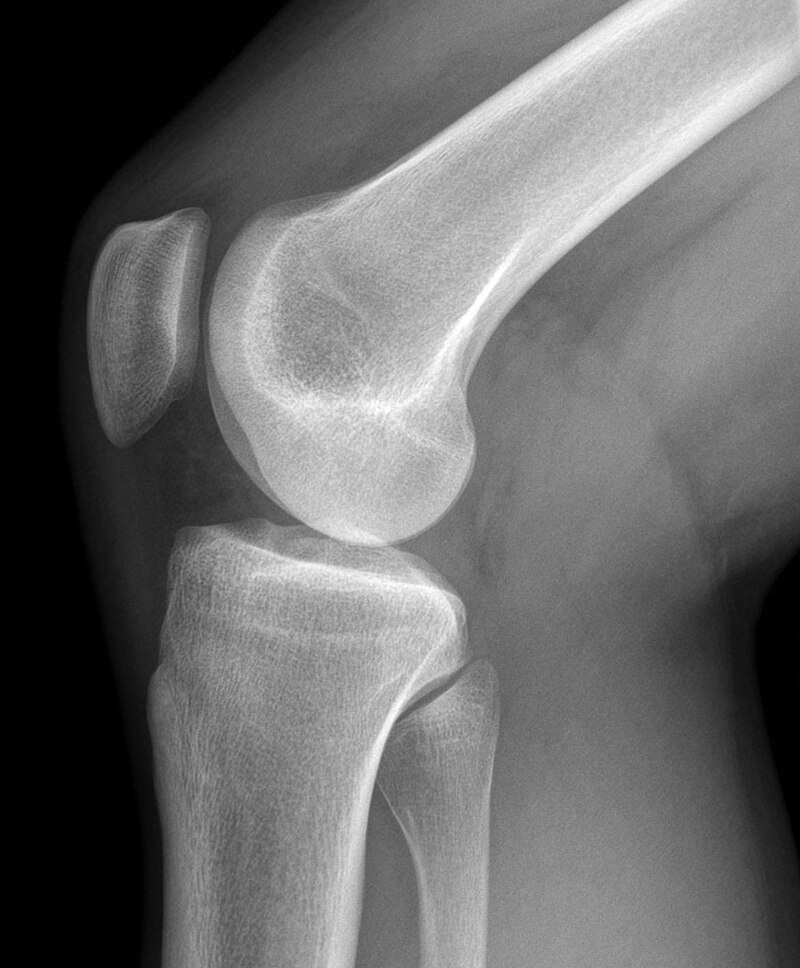
\includegraphics[width=10cm]{Knie-roentgen-r-seite} % https://upload.wikimedia.org/wikipedia/commons/thumb/8/89/Knie-roentgen-r-seite.jpg/800px-Knie-roentgen-r-seite.jpg

\section{X-ray and radiography}
\begin{itemize}
\item Radiography (X-ray 2D \popup{projection}{Radiography is also a
    projection imaging modality, meaning that each point on the image
    corresponds to information along a straight line through the
    patient}) is a transmission imaging modality where X-rays are
  emitted from a \popup{source}{An X-rays generator.}, pass through
  the patient, and are detected on the other side using a flat
  (usually \popup{digital TFT}{In digital X-ray detectors, a TFT array
    is used to read out electrical charges generated by the impact of
    the X-rays.}) detector (see
  Fig.~\ref{fig:projectional_radiography}).
\end{itemize}
\vspace{-4ex}
\begin{figure}[!h]
  \centering
  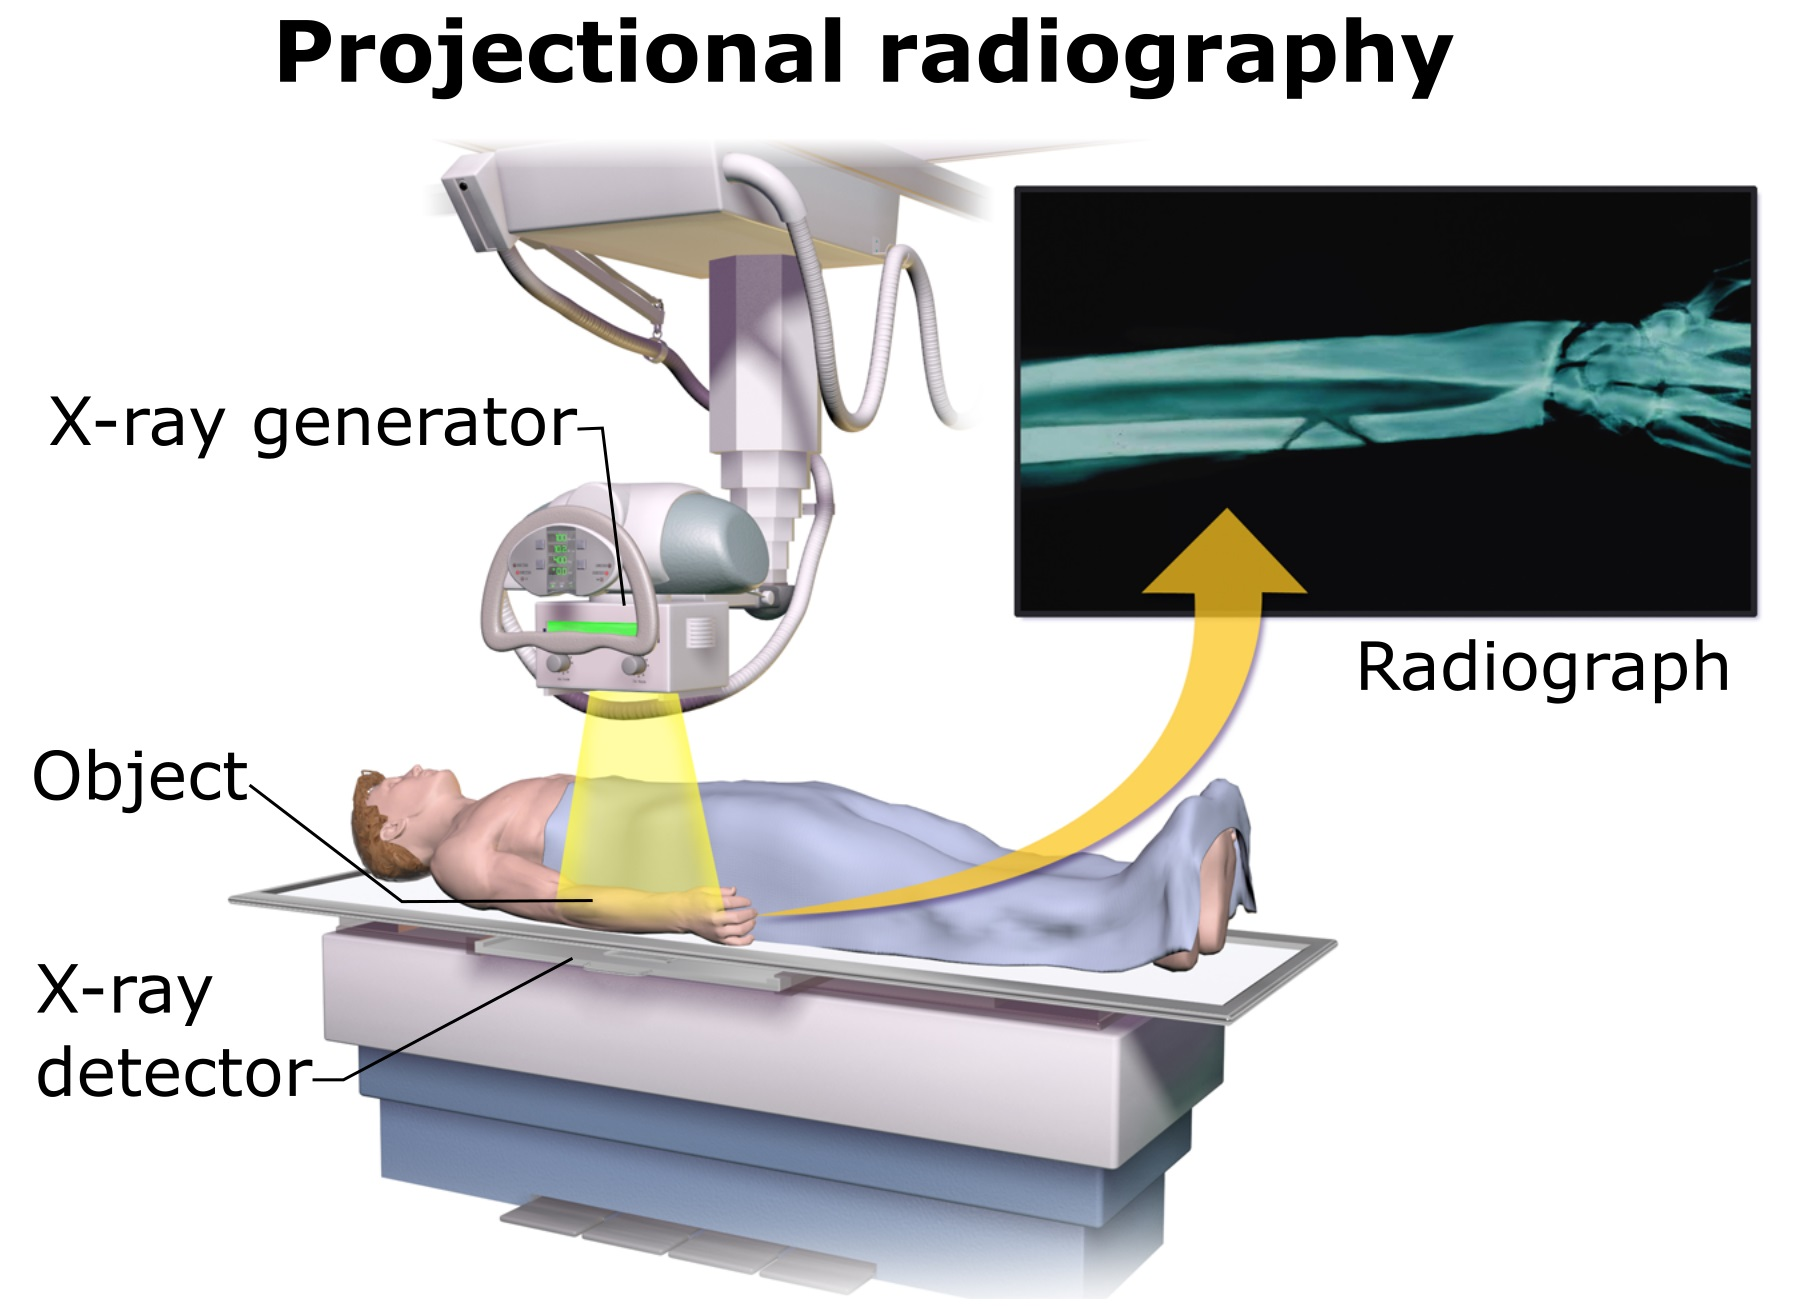
\includegraphics[width=6cm]{Projectional_radiography_components}
  \caption{Acquisition of projectional radiography, with an X-ray generator and a detector
    \cite{Wikipedia_X-ray_machine}.\label{fig:projectional_radiography}}
\end{figure}

\section{Transmission and attenuation}
\begin{itemize}
\item The X-ray attenuation of different tissues (e.g., bone, soft
  tissue, air) modify the homogeneous distribution of X-rays that
  enters the patient X-ray, forming the image in the detector
  \cite{bushberg2011essential} (see
  Fig.~\ref{fig:Attenuation-of-X-rays}).
\end{itemize}
\vspace{-3ex}
\begin{figure}[!h]
  \centering
  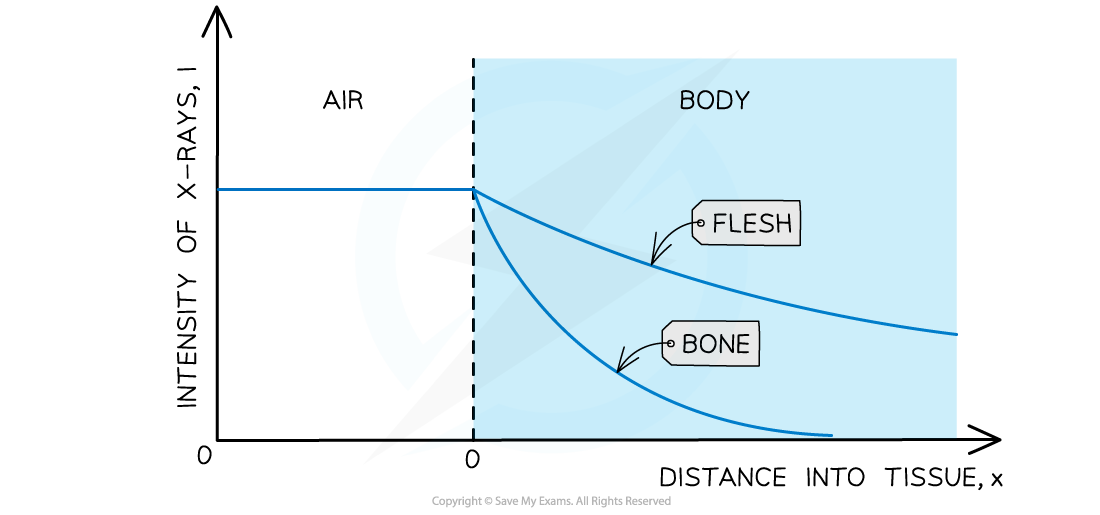
\includegraphics[width=9cm]{Attenuation-of-X-rays}
  \caption{Intensity-distance graph of X-rays for air and body
    \cite{Attenuation_X-rays}.\label{fig:Attenuation-of-X-rays}}
\end{figure}

\section{Why we are ``transparent''?}
\begin{itemize}
\item The \popup{fast ondulatory movement of X-ray-photons}{From 30
    petahertz (PHz)}{3x10$^{16}$ Hz.} to \popup{30 exahertz
    (EHz)}{3x10$^{19}$ Hz} makes them capable of \popup{penetrating
    soft tissues}{The higher the frequency of the X-rays photons, the
    higher their energy and the higher their penetration capability.}.
\end{itemize}
\vspace{-4ex}
\begin{figure}[!h]
  \centering
  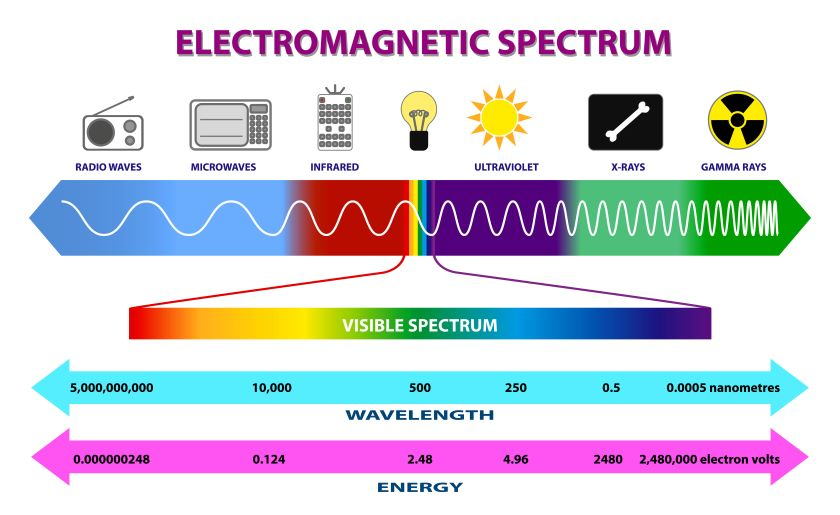
\includegraphics[width=8cm]{electromagnetic-spectrum}
  \caption{The electromagnetic spectrum
    \cite{X-rays_in_spectrum}.\label{fig:X-rays_in_spectrum}}
\end{figure}

\section{Ionization and biologic damage (1/2)}
\begin{itemize}
\item X-rays are a form of \popup{ionizing radiation}{An ionizing
    radiation is capable of removing electrons from atoms or
    molecules, a process known as ionization (when an atom or molecule
    loses or gains electrons, it acquires a net electrical charge and
    becomes an ion).} (see Fig.~\ref{fig:ionization}), creating
  \popup{free radicals}{A free radical is an atom or molecule that has
    an unpaired electron in its outer shell. Because electrons prefer
    to exist in pairs, this unpaired electron makes the free radical
    highly unstable and very reactive.}.
\end{itemize}
\vspace{-3ex}
\begin{figure}[!h]
  \centering
  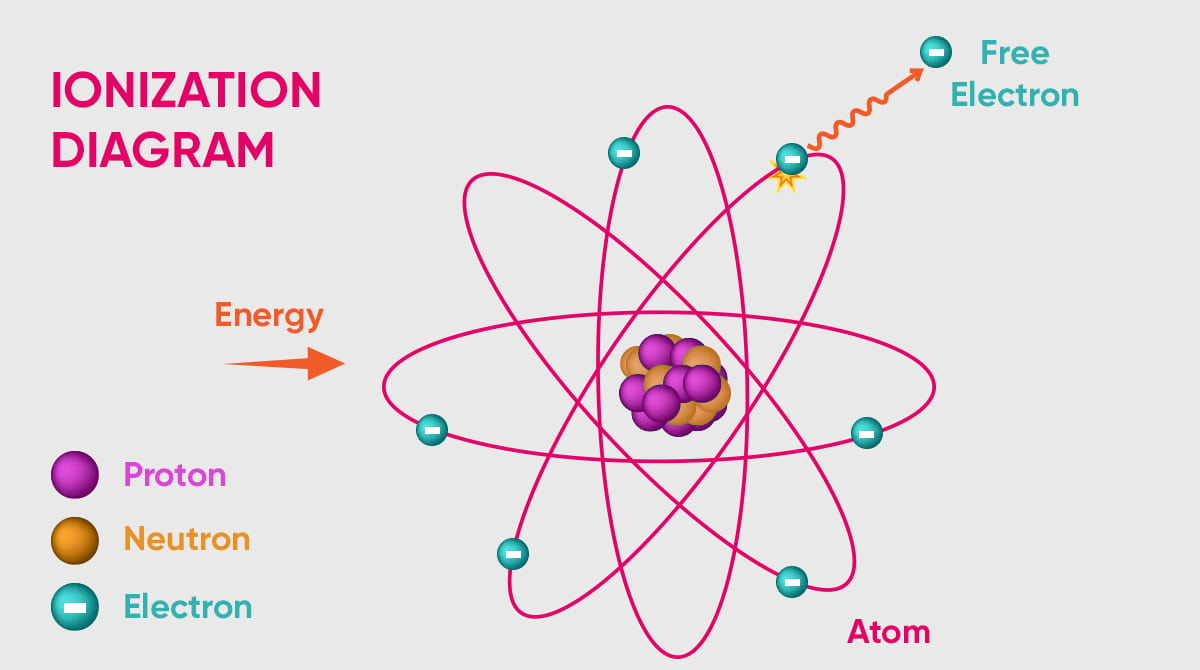
\includegraphics[width=8cm]{ionization-diagram}
  \caption{Ionization
    \cite{Perakende_ionization}.\label{fig:ionization}}
\end{figure}

\section{Ionization and biologic damage (2/2)}
\begin{itemize}
\item Free radicals are extremely reactive and can interact with
  biomolecules. This can produce a list of effects
  \cite{bushberg2011essential}:
  \begin{enumerate}
  \item \textbf{Short-term effects} (usually under high doses):
    \href{https://en.wikipedia.org/wiki/Radiation_burn}{burns},
    sickness.
  \item \textbf{Long-term effects}:Damage to DNA, could suffer
    \popup{mutations}{Although heavily irradiated cells often die
      during mitosis, preventing the propagation of seriously
      defective cells, damage to DNA at locations responsible for
      controlling cell division (e.g., oncogenes or tumour suppressor
      genes) could potentially lead to the formation of a tumour or
      cancer}, and \popup{tissue disfunction}{If there is ellular
      dysfunction, tissues can lose function and finally generate
      organ failure.}.
  \end{enumerate}
\end{itemize}

\section{Artifacts}
\begin{itemize}
\item In radiology, artifacts come from hardware failure, operator
  error (including the interaction/control with/of the patient) and
  software (post-processing) artifacts.
\item Only in digital radiology.
\end{itemize}

\section*{}
\subsection{Motion blur}
\vspace{-4ex}
\begin{figure}[!h]
  \centering
  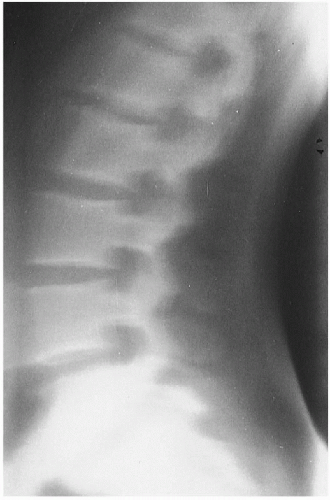
\includegraphics[width=3.5cm]{motion_blur_2}
  \caption{The image unsharpness was caused by patient movement
    \cite{radiology_key}.\label{fig:motion_blur}}
\end{figure}

\section*{}
\subsection{Static electricity}
\vspace{-3ex}
\begin{figure}[!h]
  \centering
  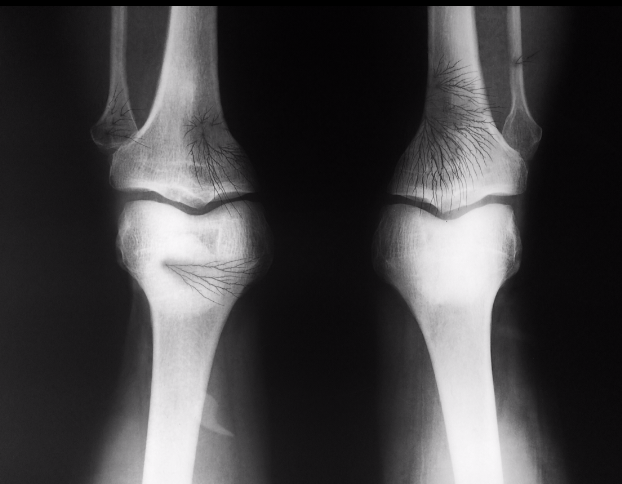
\includegraphics[width=7cm]{static-electricity}
  \caption{\cite{radiopaedia}.\label{fig:static_electricity}}
\end{figure}

\section*{}
\subsection{Dead pixel}
\vspace{-3ex}
\begin{figure}[!h]
  \centering
  \begin{tabular}{cc}
    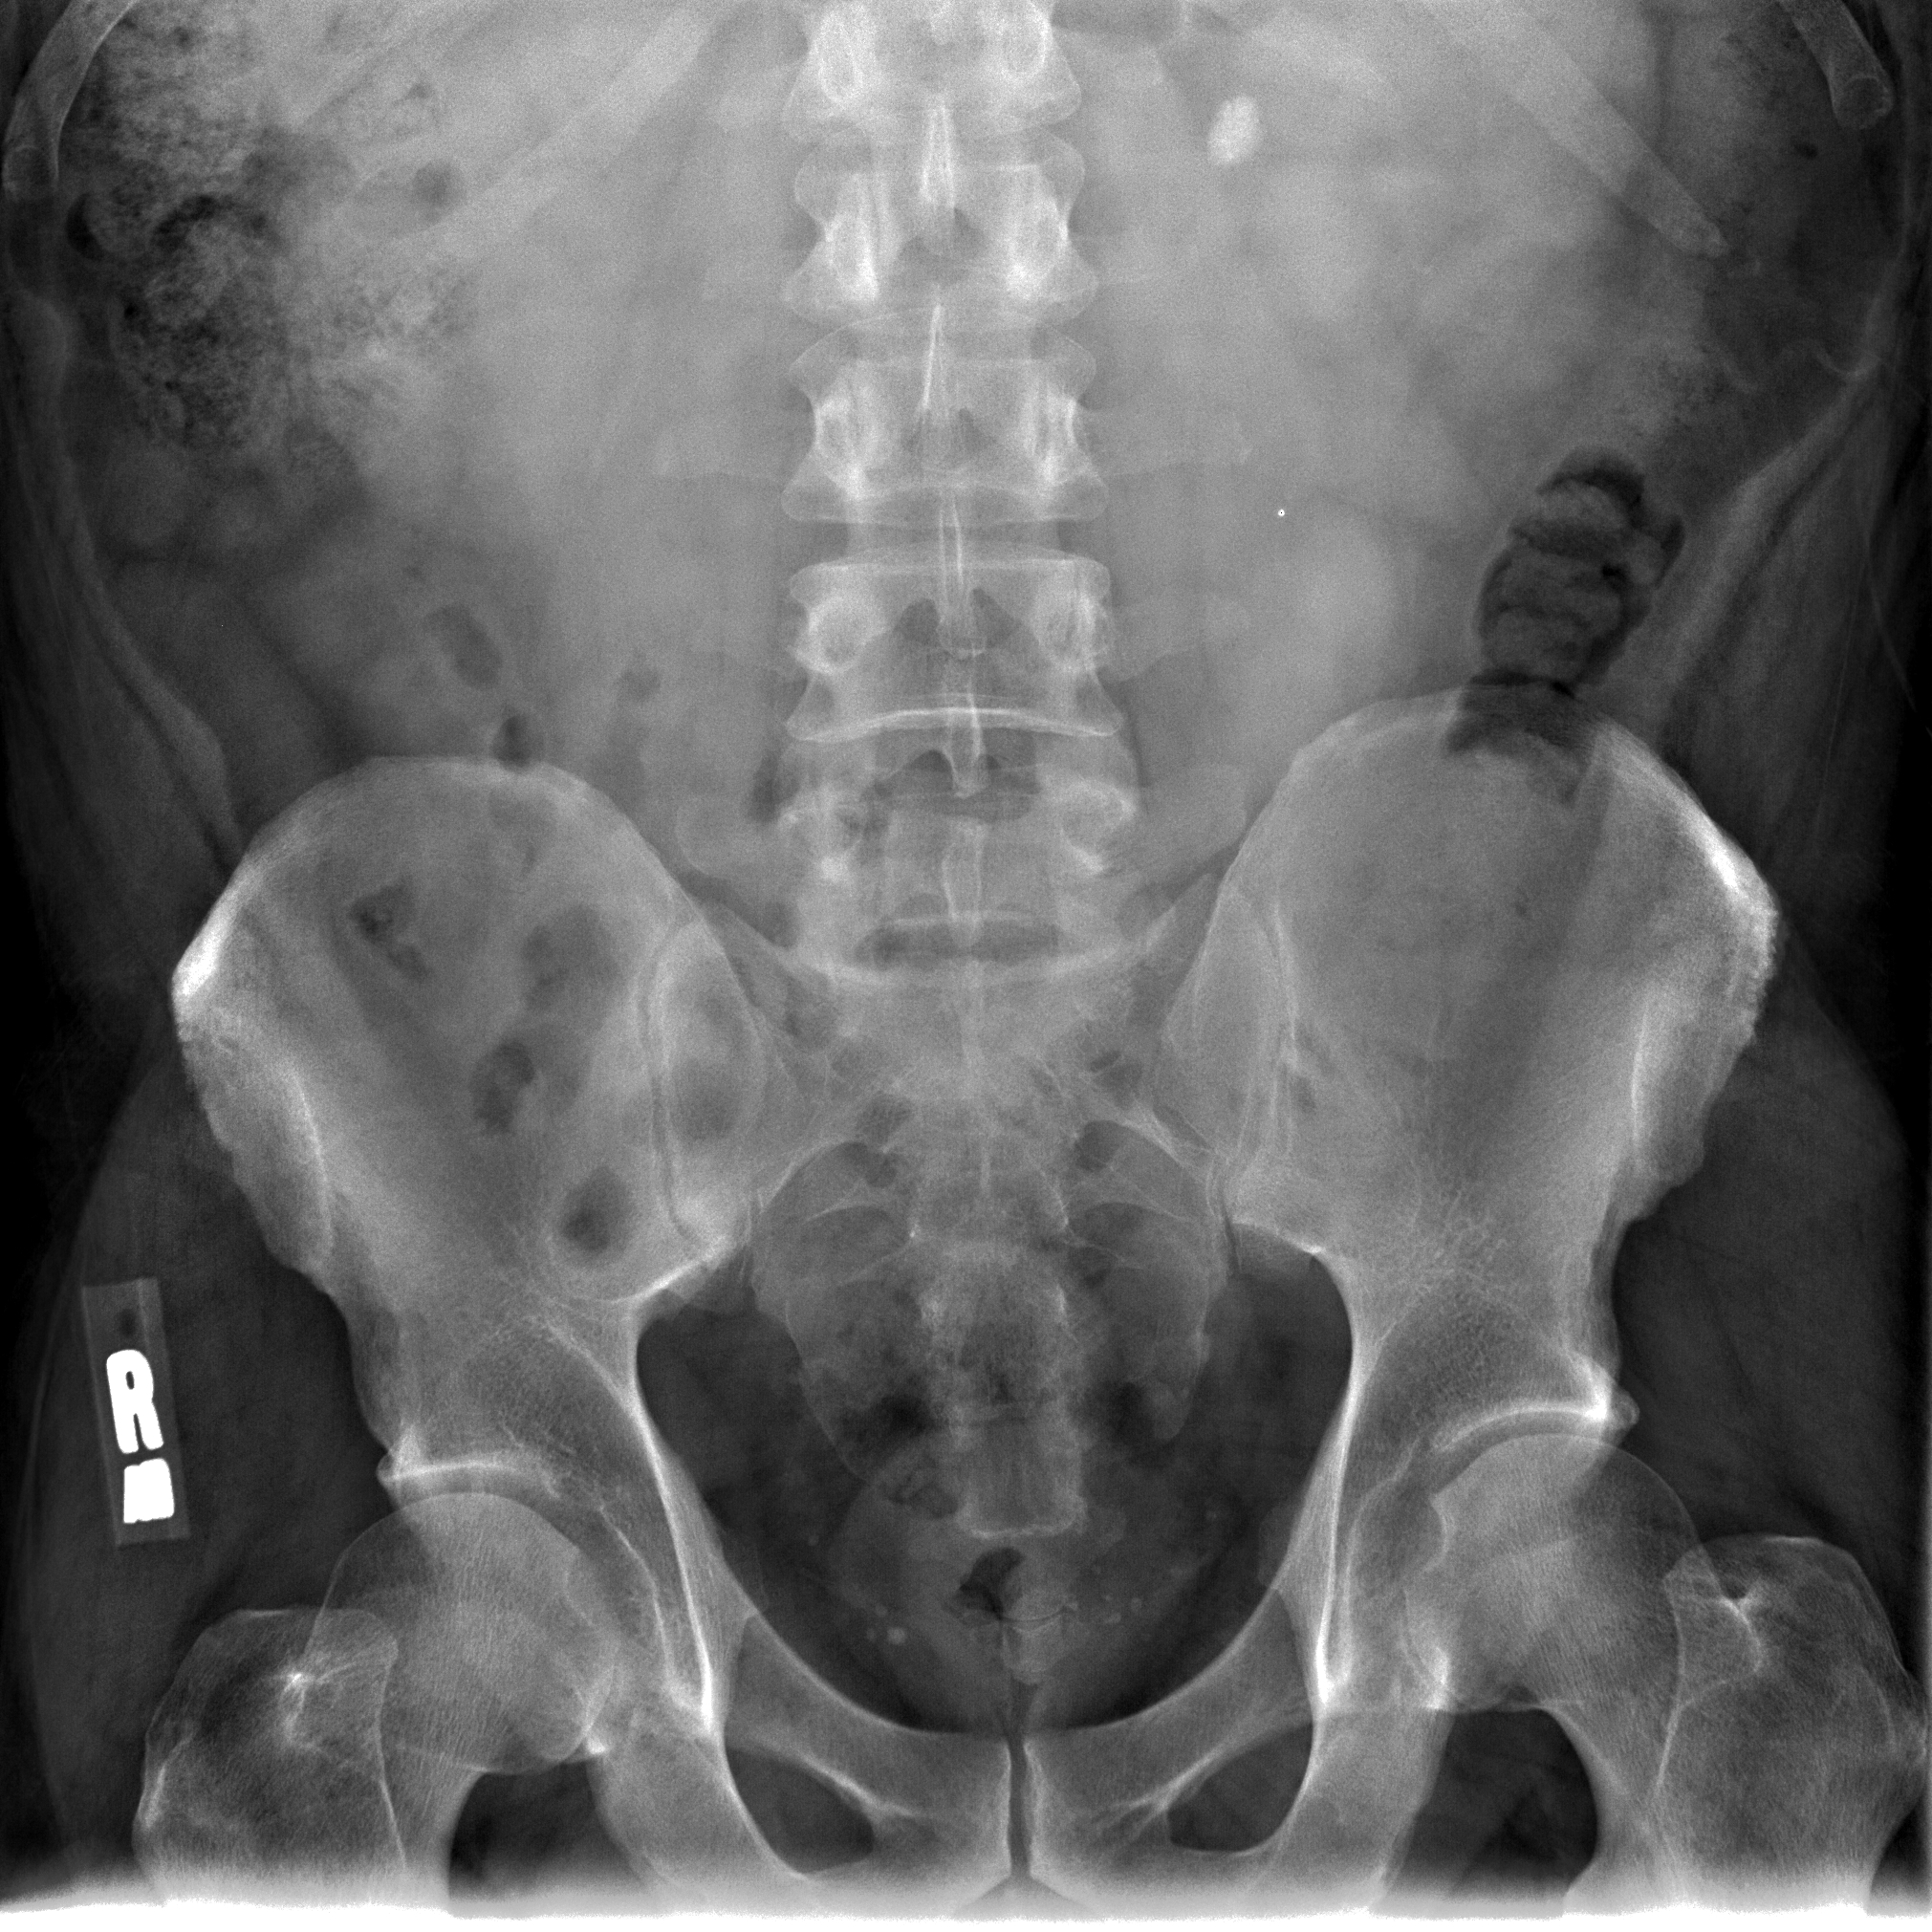
\includegraphics[width=5cm]{dead-pixel-artifact_frontal} &
                                                               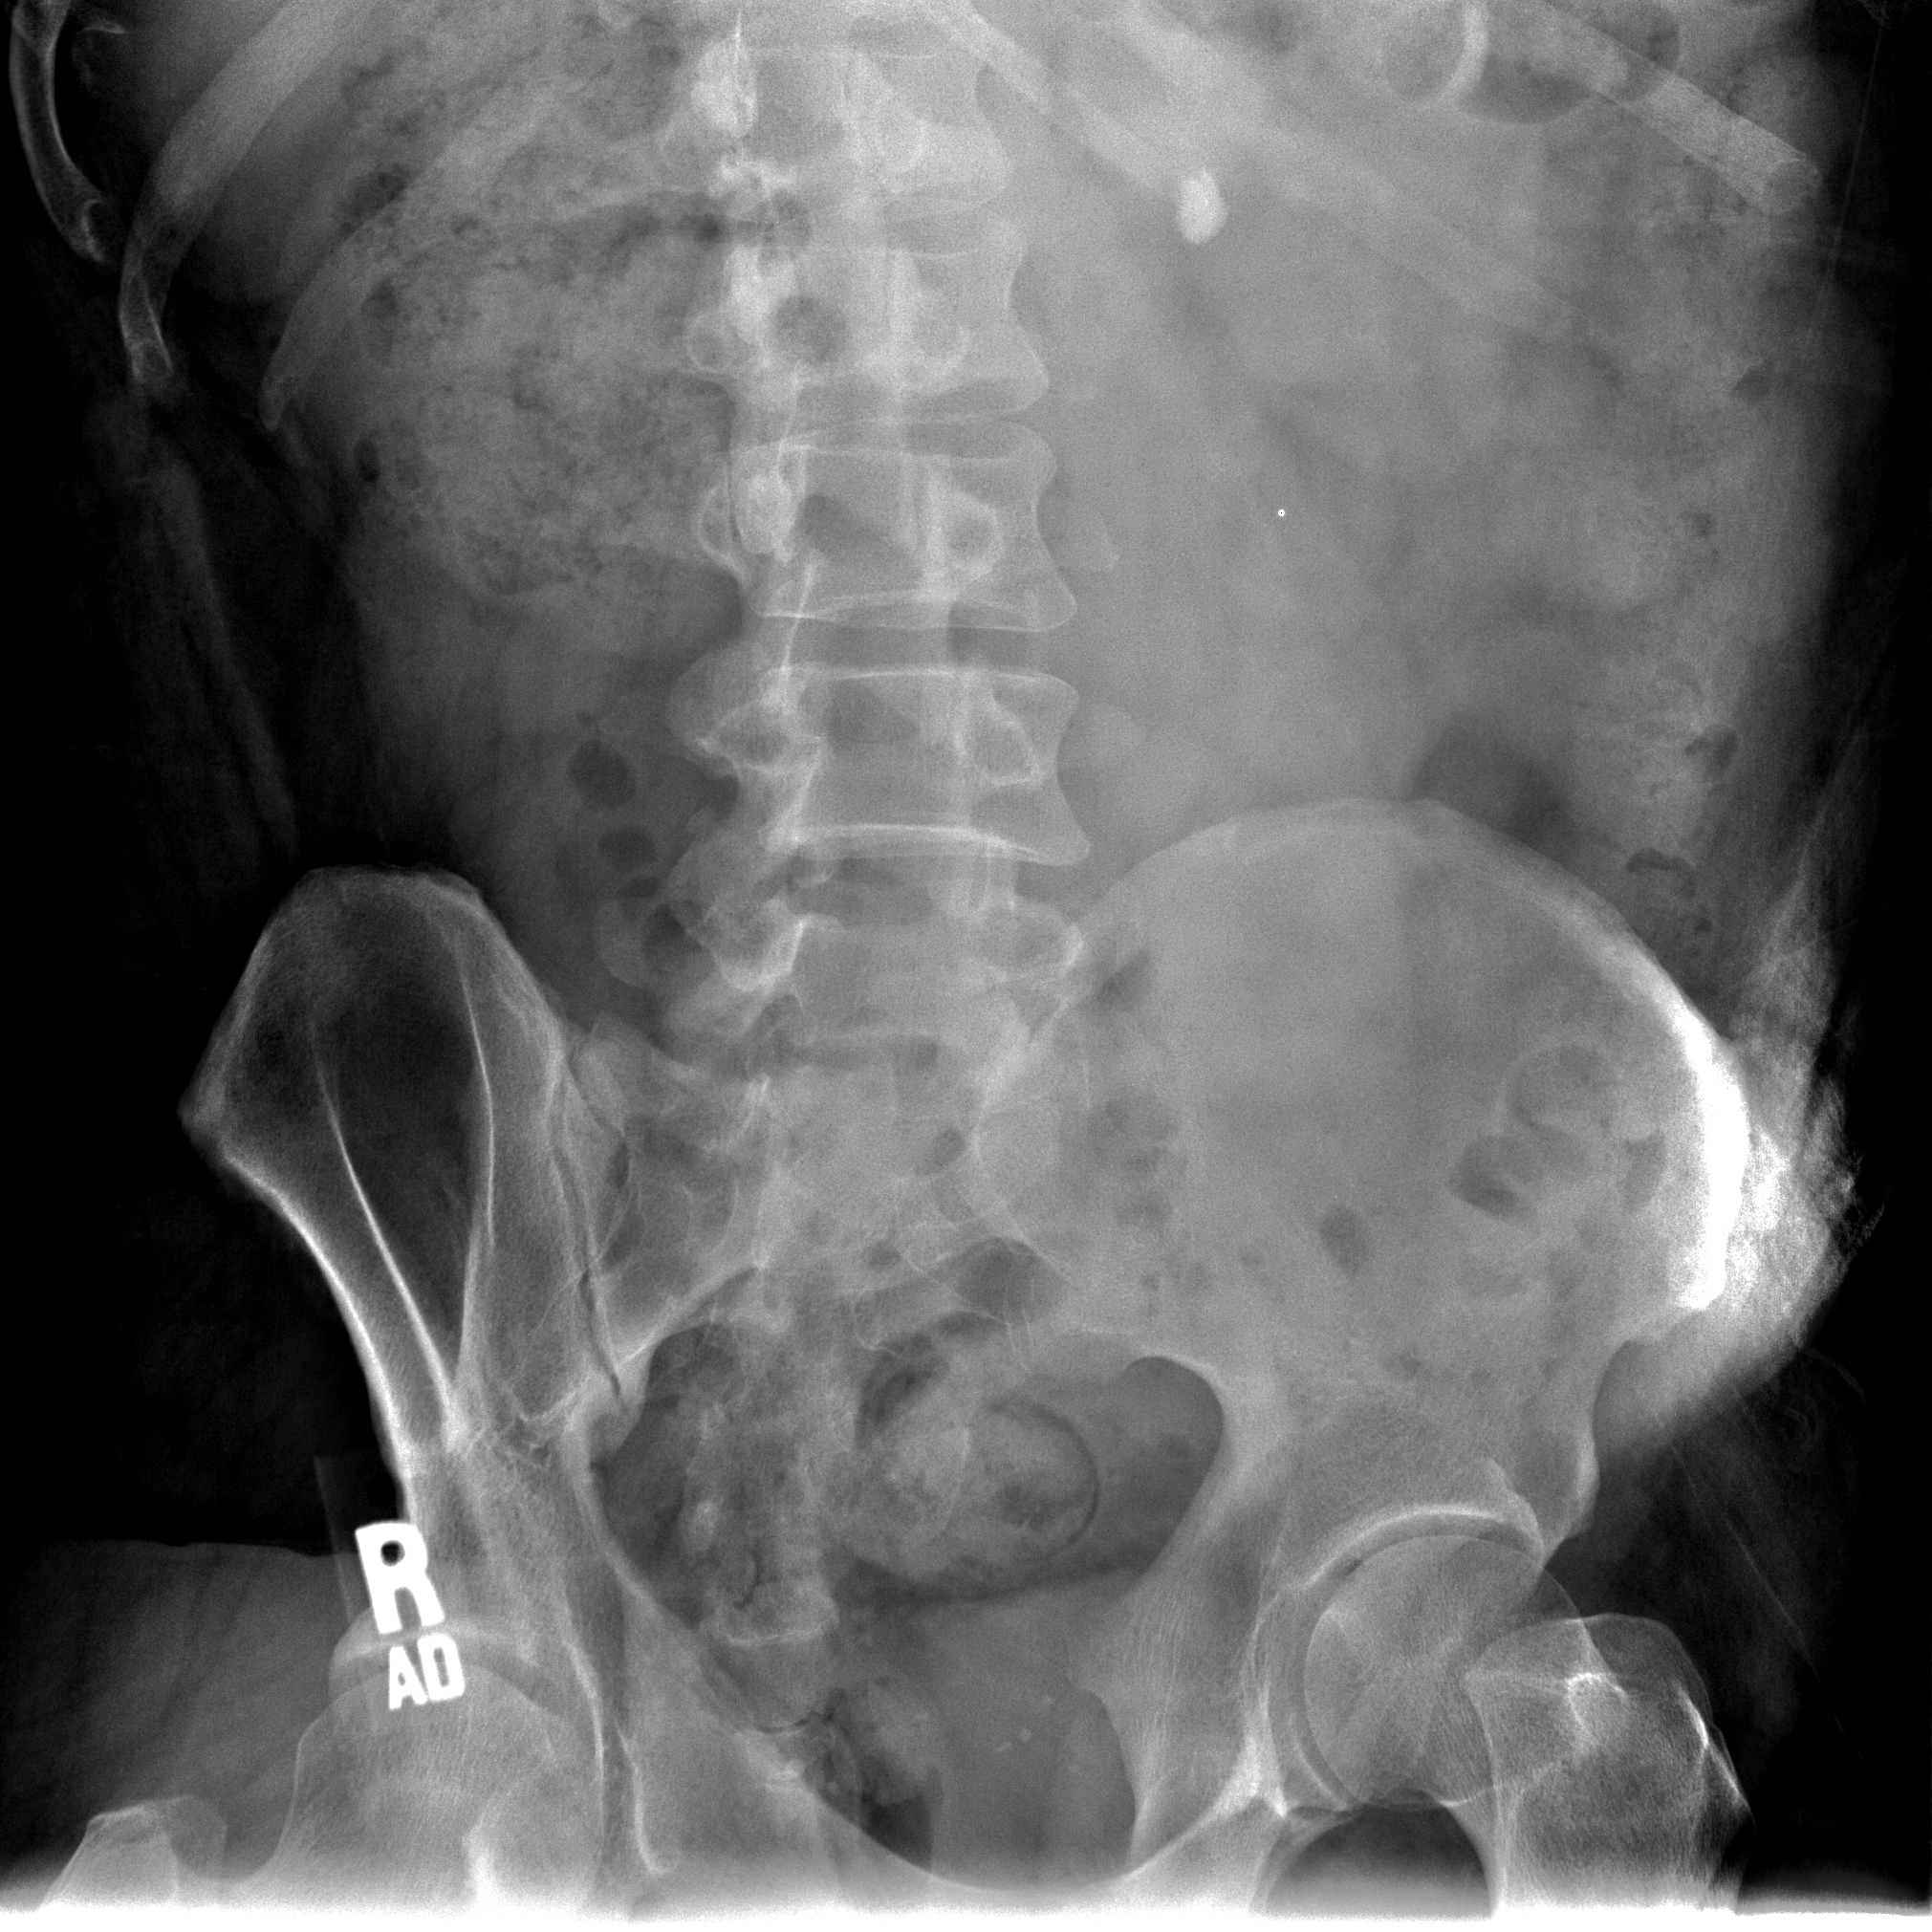
\includegraphics[width=5cm]{dead-pixel-artifact_oblique}
  \end{tabular}                                                
  \caption{\cite{radiopaedia}.\label{fig:dead_pixel}}
\end{figure}

\section*{}
\subsection{Under- and over-exposure}
\begin{itemize}
\item In digital radiology (down), the detector always generates a good contrast.
\item The main drawback is that, under-exposure usually have more noise.
\end{itemize}
\vspace{-4ex}
\begin{figure}[!h]
  \centering
    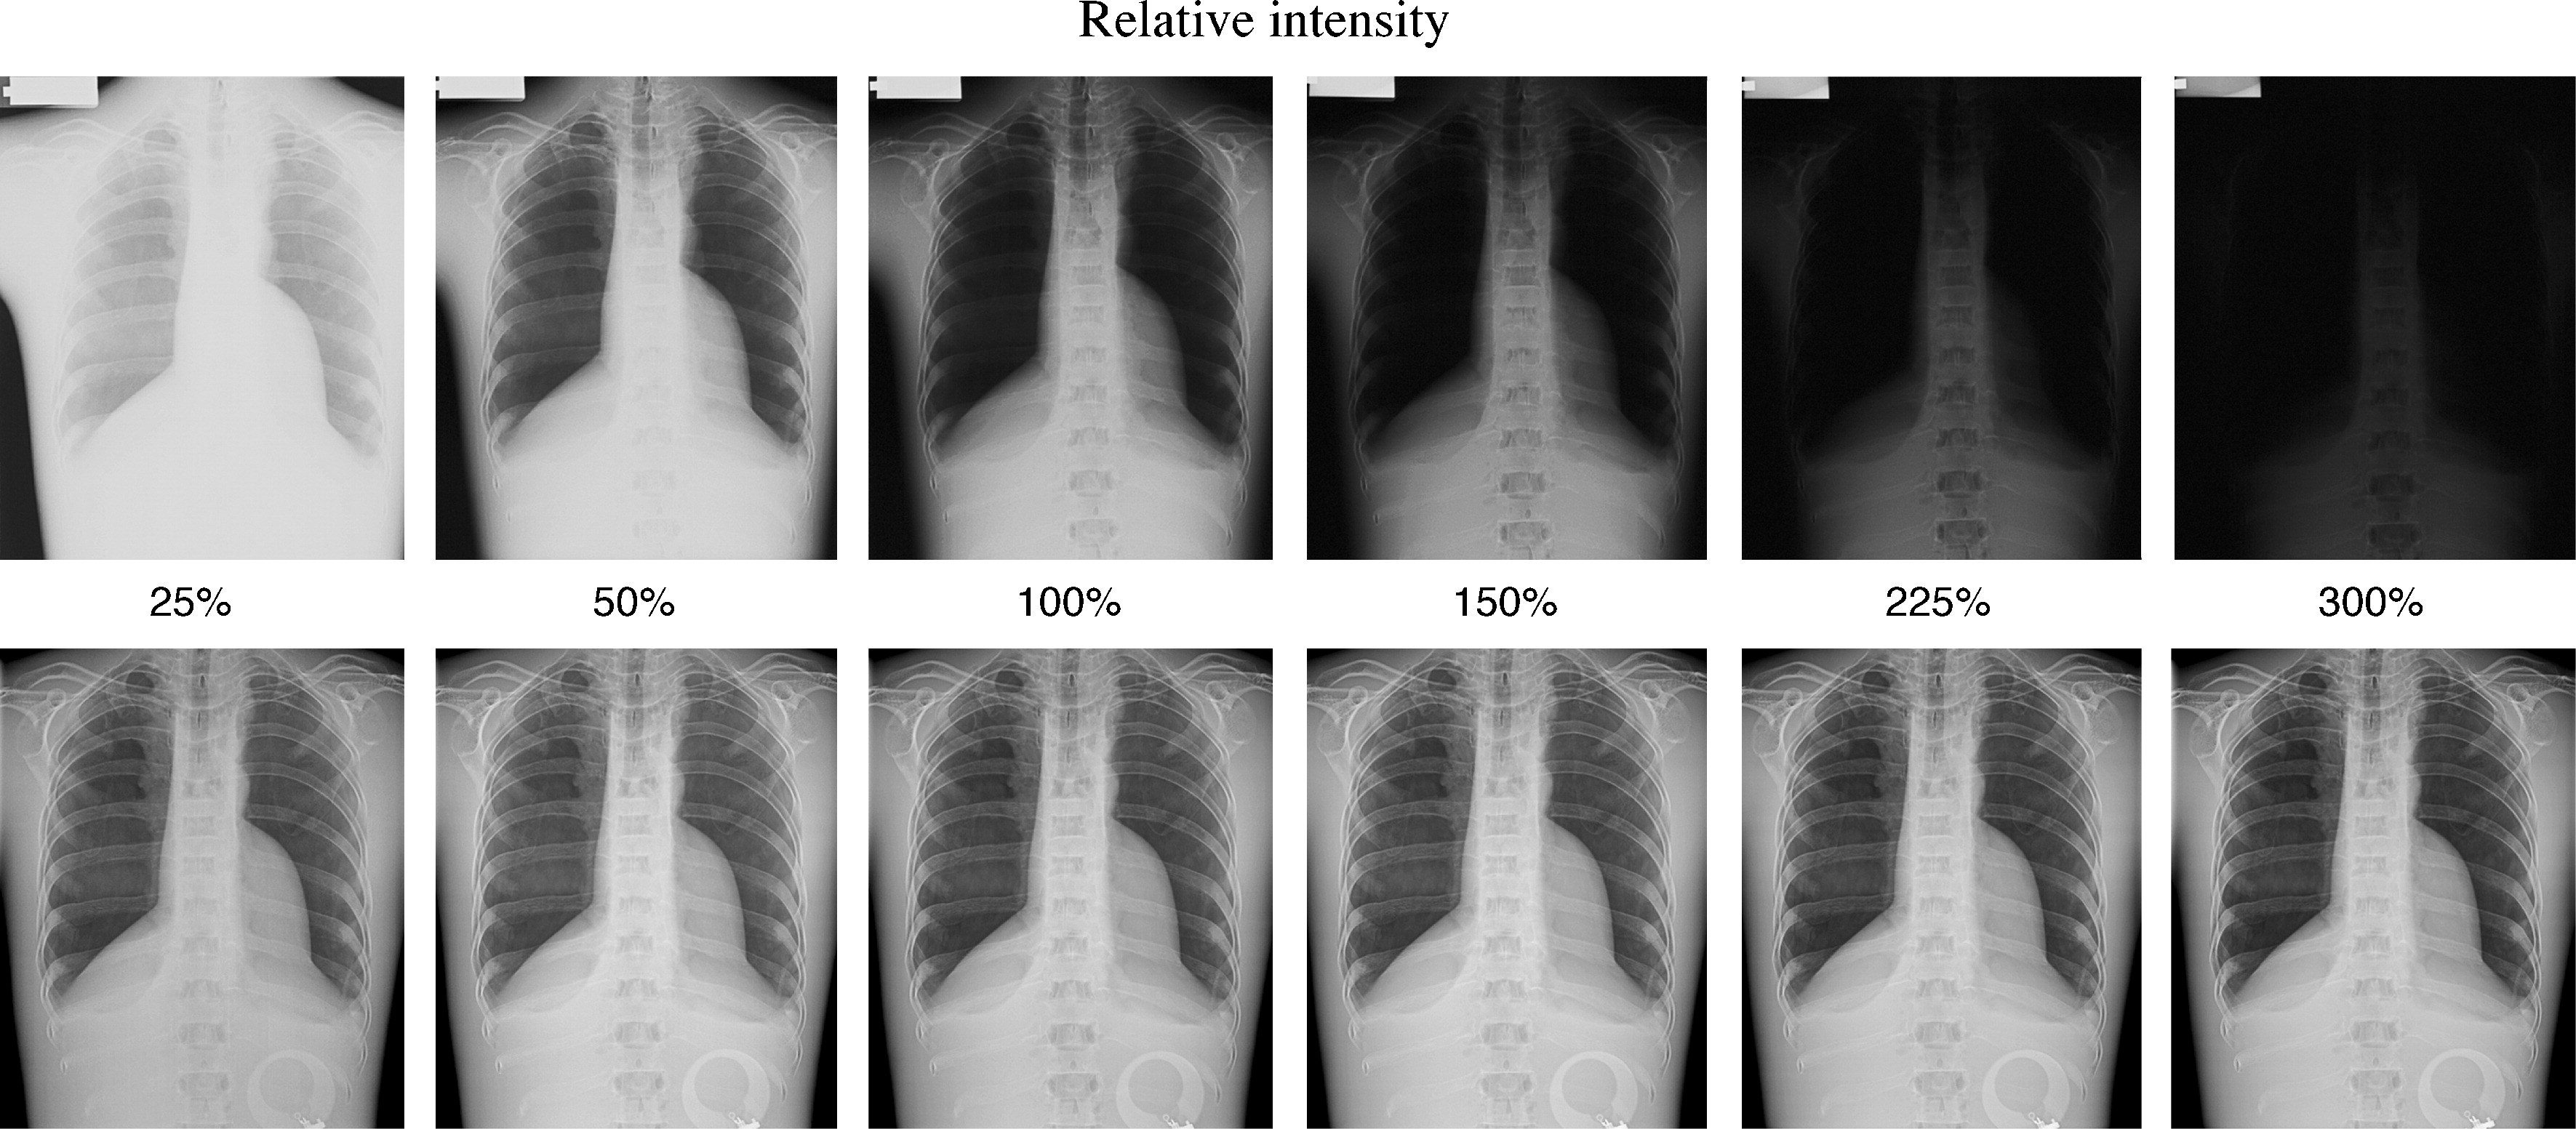
\includegraphics[width=9cm]{X-ray_exposure}
    \caption{Exposure impact (up: analog, down: digital)
      \cite{VELDKAMP2009209}.\label{fig:exposure}}
\end{figure}

\section{Mammography}
\begin{itemize}
\item Mammography is the 2D X-rays projection\\ of the breast
  \cite{bushberg2011essential}.
\item Makes use of much lower x-ray energies\\ than general purpose
  radiography.
\end{itemize}
\vspace{-20ex}
\begin{figure}[!h]
  \begin{flushright}
    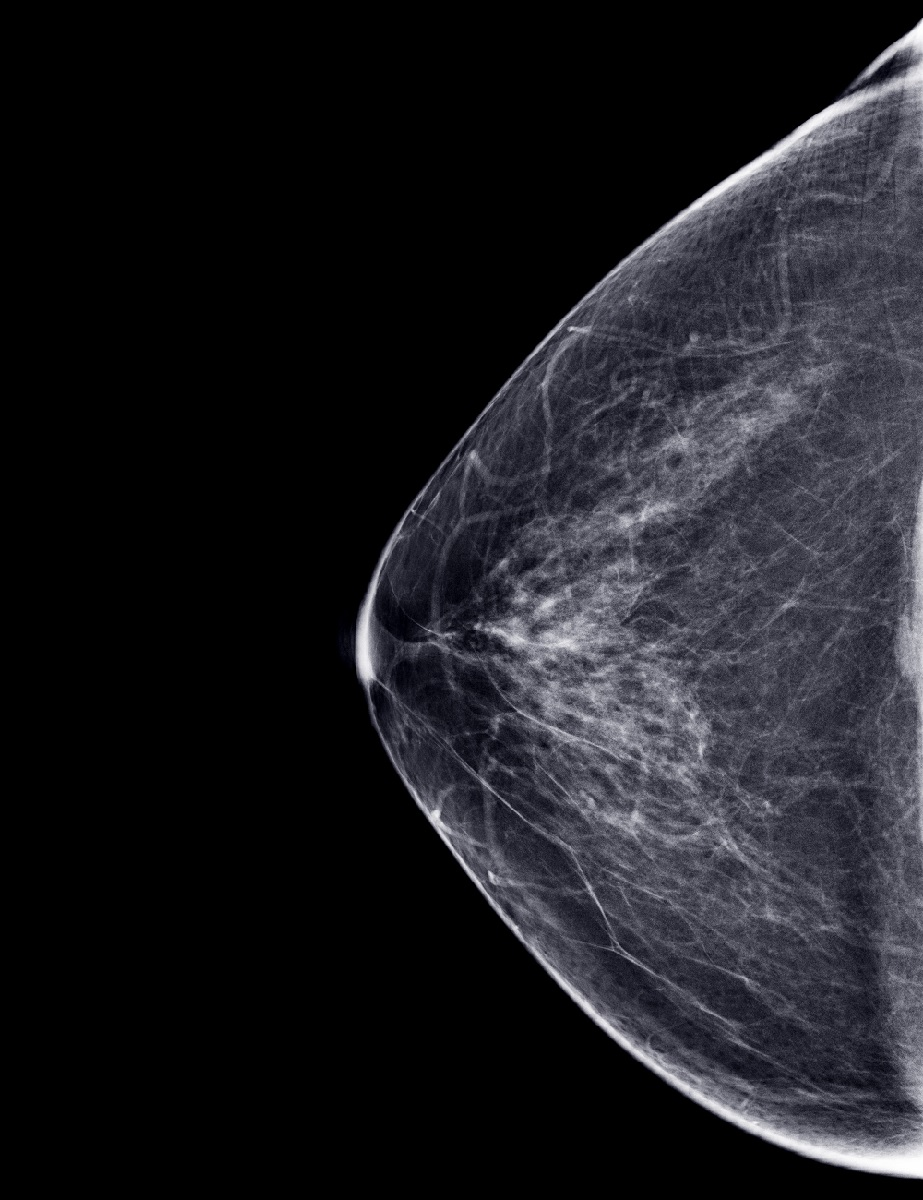
\includegraphics[width=4.5cm]{normal_mammogram}
    \end{flushright}
    \caption{Mamogram \cite{CDC_mammograms}.\label{fig:mamogram}}
\end{figure}

\section{Fluoroscopy}
\begin{itemize}
\item A fluoroscope produces real-time X-ray images with high temporal
  resolution (e.g., 30 frames per second), allowing continuous motion
  viewing, useful for \popup{interventional procedures}{Fluoroscopy is
    used for positioning catheters in arteries, visualizing contrast
    agents in the \gls{GI} tract, and for other medical applications
    such as invasive therapeutic proce- dures where real-time image
    feedback is necessary. It is also used to make x-ray movies of
    anatomic motion, such as of the heart or the esophagus.}
  \cite{bushberg2011essential}.
\item Compared to ``one-shot'' radiography, the images are more noisy.
\item
  \href{https://en.wikipedia.org/wiki/Fluoroscopy#/media/File:Normal_barium_swallow_animation.gif}{Swallowing
    of varium} \cite{Wikipedia_Fluoroscopy}.
\end{itemize}

\section{Quantum noise}
\begin{itemize}
\item Quantum noise is the most common noise in X-rays imaging.
\item It is directly related to photon counting (fewer photons
  $\rightarrow$ more noise).
\item More evident (lower \gls{SNR}) at low radiation doses.
\end{itemize}
\vspace{-4ex}
\begin{figure}[!h]
  \centering
    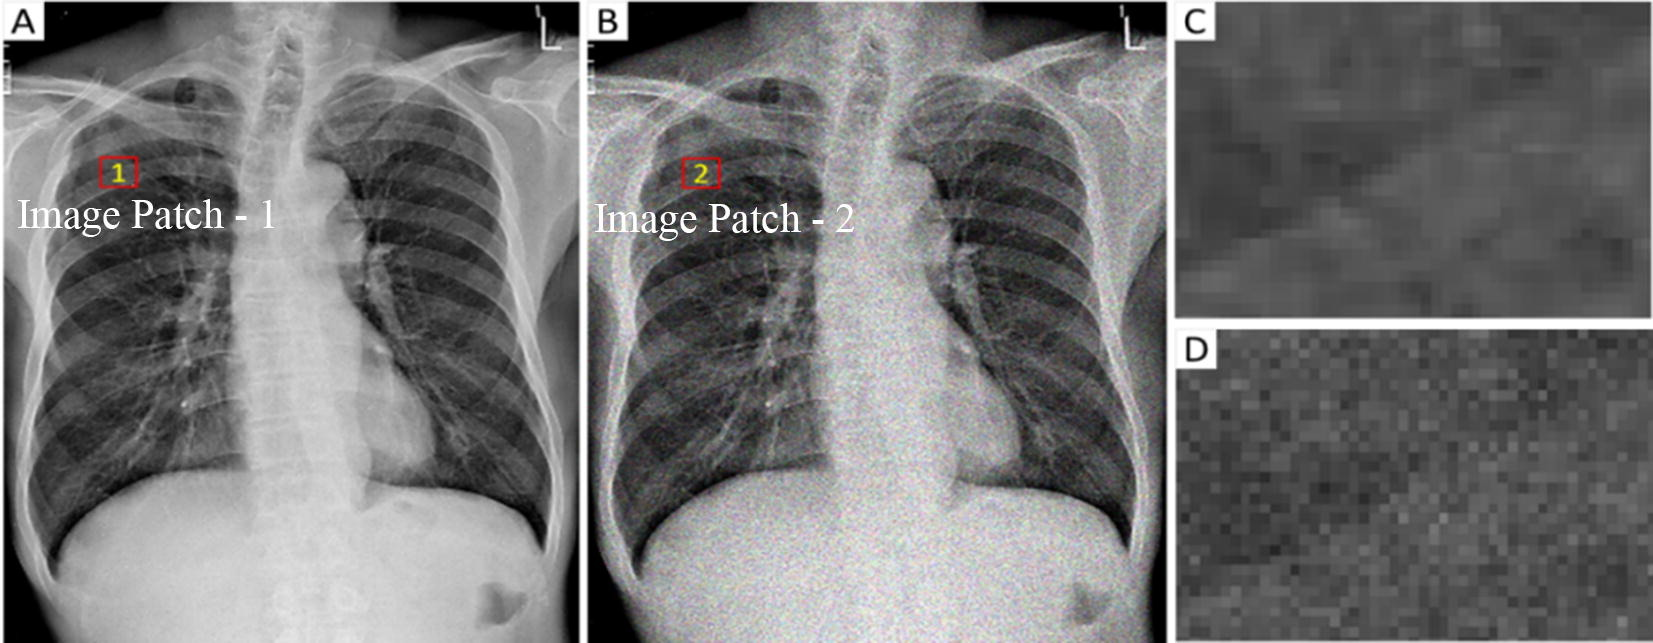
\includegraphics[width=10cm]{quantum_noise_X-rays}
    \caption{Quantum noise in radiology
      \cite{CHANDRA2020107426}.\label{fig:quantum_noise_X-rays}}
\end{figure}
